
\begin{figure}[!ht]
\centering
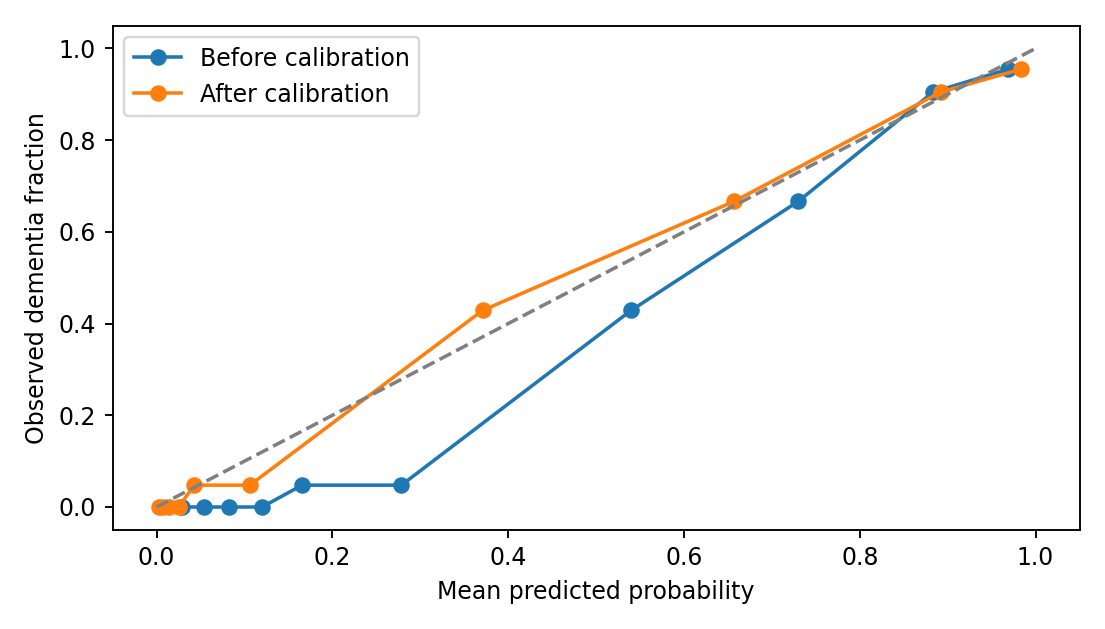
\includegraphics[width=.86\linewidth]{figures/calibration_before_after.png}
\caption{Calibration of the shared final predictor before and after sigmoid adjustment on the same 212 held-out validation participants. Each curve uses ten quantile bins. The dashed diagonal marks perfect agreement.}
\label{fig:ritam-calibration}
\end{figure}

Each point compares the mean predicted probability in a bin with the fraction of participants in that bin who developed dementia within five years. Points below the diagonal indicate overprediction and points above it indicate underprediction \cite{vancalster}. Before adjustment, several low and intermediate probability bins lie below the diagonal. After adjustment, the curve is generally closer to the diagonal, although gaps remain in some bins. On these same held-out participants, the Brier score, the mean squared error of the predicted probabilities, decreased from 0.0771 to 0.0669.

The 211-person calibration partition was used to fit the sigmoid and choose the cutoff of 0.513078. The figure uses the separate validation partition to assess probability agreement. The cutoff then converts each calibrated probability into a binary flag for reporting precision, recall and $F_1$.
